\section{Data}

The German electricity market was liberalized in 1998 and is the largest in Europe with a gross production of 633.2 TWh in 2006 \citep{IEA2007}. More than half of the power is generated with coal, other major sources are nuclear and gas. The German power market is dominated by a few large players (E.ON, RWE, EnBW, Vattenfall). These firms are both transmission system operators and own 90\% of total generation capacity. \cite{Brunekreeft2006} report values for the Herfindahl Hirschman Index (HHI)\footnote{This is a common measure of market power and is calculated as sum of the squared market shares in an industry.} of over 2000. Electricity distribution is organized by approximately 900 communal distributors. The German energy market regulator  \emph{Bundesnetzagentur} was installed in 2005. There are several interesting developments on the German electricity market. There is an urgent need for new capacities as Germany decided on a phase-out of nuclear power generation by 2020 (\cite{IEA2007a}). In addition to that, a large stake of the existing generation capacities are close to the end of its service life. The \emph{German Energy Agency} estimates that investments in generation capacity of up to 40,000 MW will be necessary, see Fig. \ref{fig:nuclear}. This, together with a tendency towards more environmental-friendly technologies supports the importance of exploring investment incentives. The Question is whether there will be enough and efficient investments.
Another interesting development is the introduction of significant wind generation, especially in the northern part of germany. Wind installations reached 15\% of total capacity installed in 2005 and will grow further (\cite{IEA2007a}). The capcity factor of wind however, ist just at 17\% meaning that it�s low and uncertain availablity adds to overall unvertainty.
In the last years, the price levels on German wholesale electricity markets have been rising as reported by \cite{Weigt2007} who attribute this development to market power. In a similar argument, \cite{Brunekreeft2005} argues that this rising prices are the result of market power of the "`Big Four"' which is now exercised on wholesale markets as transmission tariffs (the big four are vertically integrated) came under increased regulatory pressure.

\begin{table}[htb]
\centering
\scriptsize
\caption{Transfer capacities (Winter 2006/07) and congestion (Jan-May 2005)}
\vspace{0.3cm}
% Table generated by Excel2LaTeX from sheet 'Tabelle1'
\begin{tabular}{lrrrrr}
\hline
           &            & \multicolumn{ 2}{c}{to Germany} & \multicolumn{ 2}{c}{from Germany} \\
\hline
           &            & Capacities & \% of hrs.  & Capacities & \% of hrs.  \\

           &            &            &  congested &            &  congested \\
\hline
\hline
   Austria &            &       1400 &        0\% &       1600 &        0\% \\

Czech Republic &            &       2260 &       68\% &        700 &       36\% \\

Switzerland &            &       4000 &            &       2400 &        1\% \\

    France &            &       2850 &       33\% &       3300 &       41\% \\

Netherlands &            &       3000 &       64\% &       3800 &       90\% \\

   Denmark &            &       1750 &            &       1350 &      100\% \\

    Poland &            &       1100 &            &       1200 &            \\

    Sweden &            &        600 &            &        600 &            \\
\hline
\end{tabular}  
\label{tab:transfer}
\\
\vspace{0.3cm}
\scriptsize Source: \cite{IEA2007a}
\end{table}

Apart from that, our analysis will abstract from vertical relationships and transmission constraints. According to \cite{IEA2007a}, there are no significant congestions within Germany. Cross boarder transfer capacities and congestions, which are given in table \ref{tab:transfer} there help us to determine the relevant market.

Efficiency Programs

\begin{figure}[htb]
  \centering
\caption{Estimated nuclear power capacity, 2007 to 2023}
 % 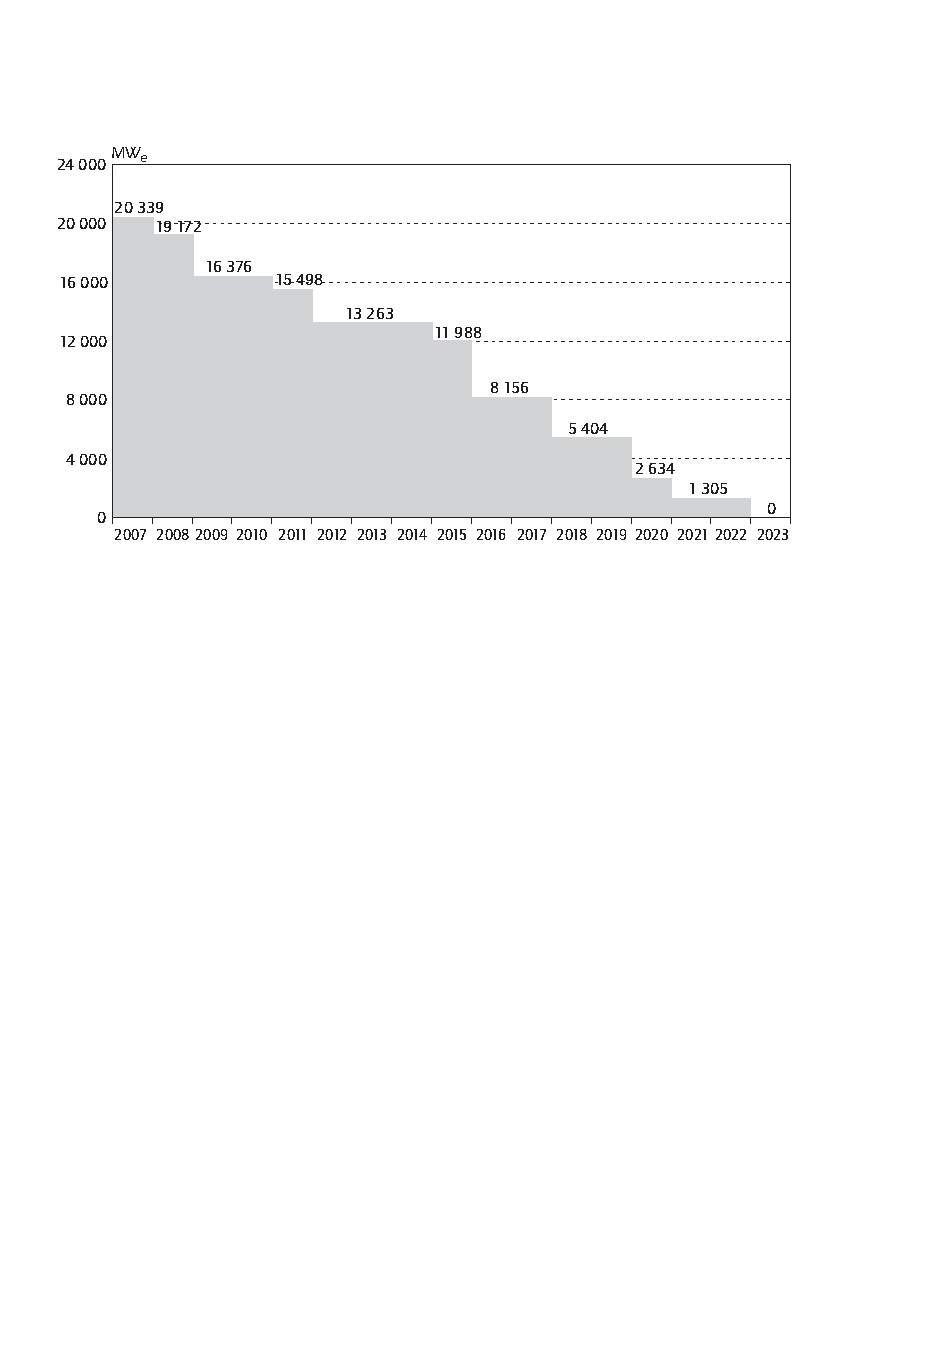
\includegraphics[width=.7\textwidth]{germandata/nuclear.pdf}
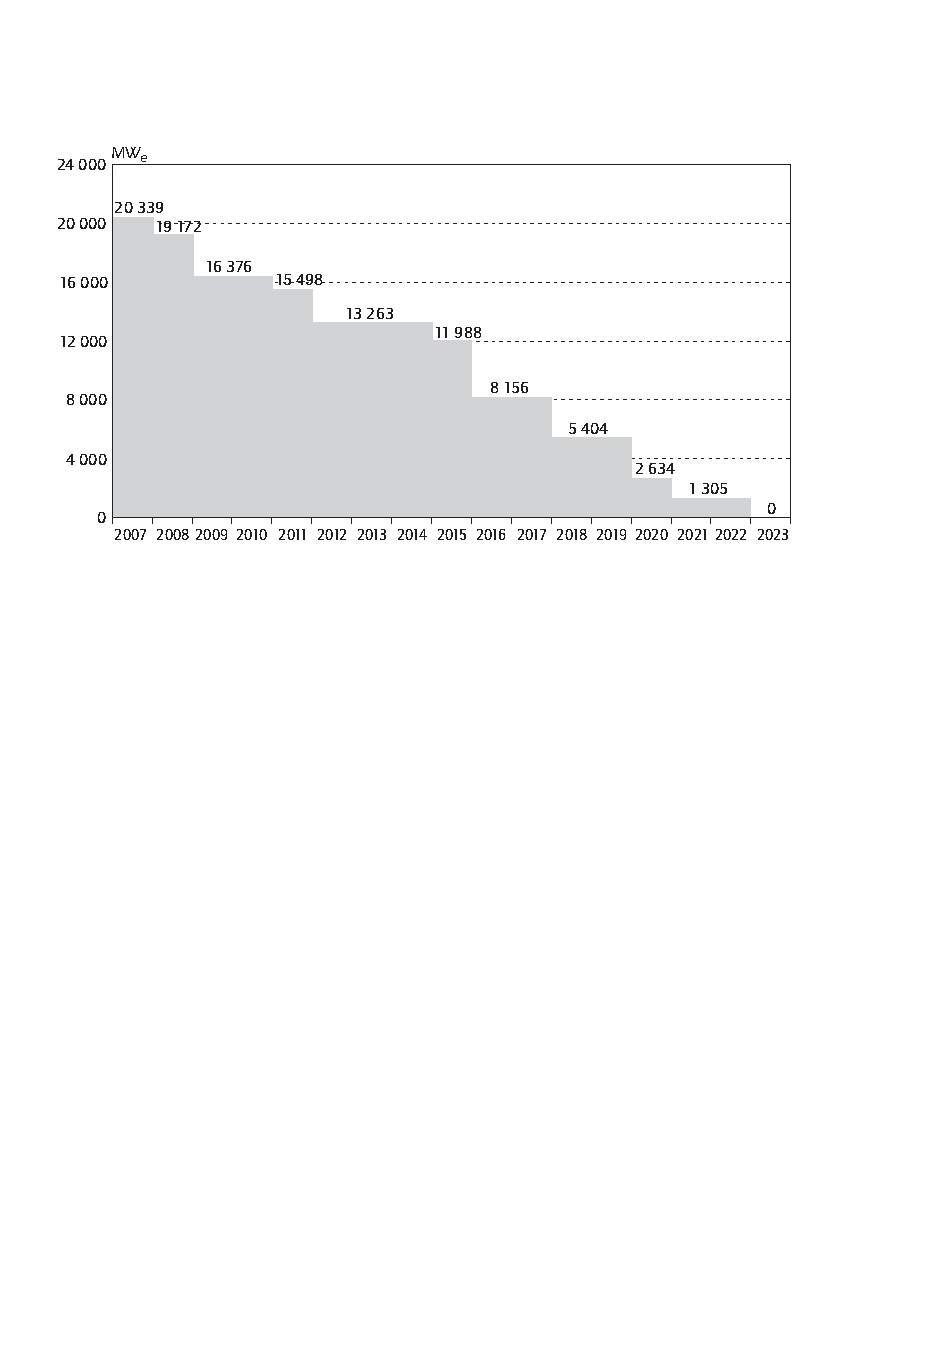
\includegraphics[width=3.5in]{germandata/nuclear.pdf}
  \label{fig:nuclear}
\\
 \scriptsize Source: \cite{IEA2007a}
\end{figure}

Tab. \ref{tab:majorcapacities} gives an overview about the existing installed capacity in different technologies.

\begin{table}[htb]
\centering
\scriptsize
\caption{Installed capacities in MW of major players in Germany}
\vspace{0.3cm}
\begin{tabular}[htb]{crrrrrrrrr}
\hline
           &      Hydro &    Nuclear &  Soft coal &  Hard coal &        Gas &        Oil &     Pumped \\
\hline\hline
       RWE &        741 &       5,499 &      10,554 &       7,249 &       4,297 &        188 &        793 \\

      E.ON &       1,320 &       8,473 &       1,425 &       9,461 &       3,808 &       1,779 &       1,110 \\

Vattenfall &          9 &       1,421 &       6,932 &       1,729 &        870 &       1,429 &       2,883 \\

      EnBW &        447 &       4,272 &        453 &       3,288 &       1,083 &        617 &        368 \\
\hline
\end{tabular} 
\label{tab:majorcapacities}
\\
\vspace{0.3cm}
\scriptsize Source: \cite{Ellersdorfer2005}
\end{table}

%Figure \ref{fig:investcosts} contains investment costs for different technologies.

%\begin{figure}[htb]
%  \centering
%\caption{Levelised costs for generation units starting commercial operation in 2015}
%  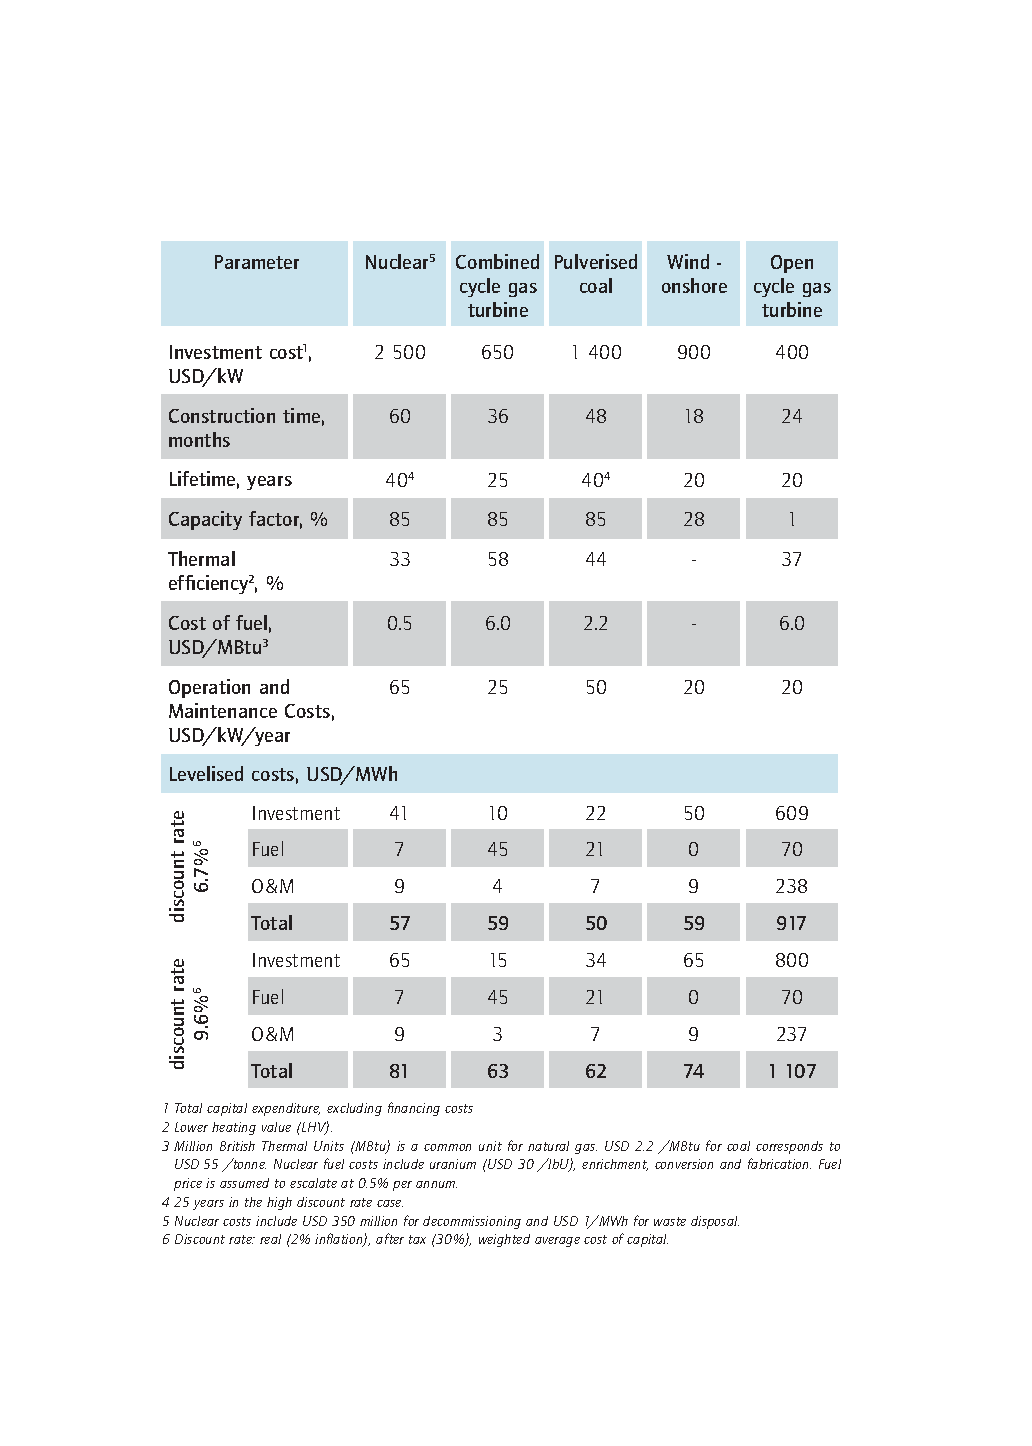
\includegraphics[width=.5\textwidth]{germandata/investmentcosts.pdf}
%  \label{fig:investcosts}
%\\
% \scriptsize Source: \cite{IEA2007c}
%\end{figure}

The major stake of electricity trading is done in OTC markets for which it is hard to obtain data. Prices from the European Energy Exchange (EEX) can be used as a good approximation. Plotting the prices against the trading volumes does not show a strong correlation. We see the expected positive relationship when comparing the exchange prices to the actual electricity demand per hour, see Fig. \ref{fig:pricequant}

\begin{figure}[htb]
  \centering
\caption{Price-quantity relationship}
  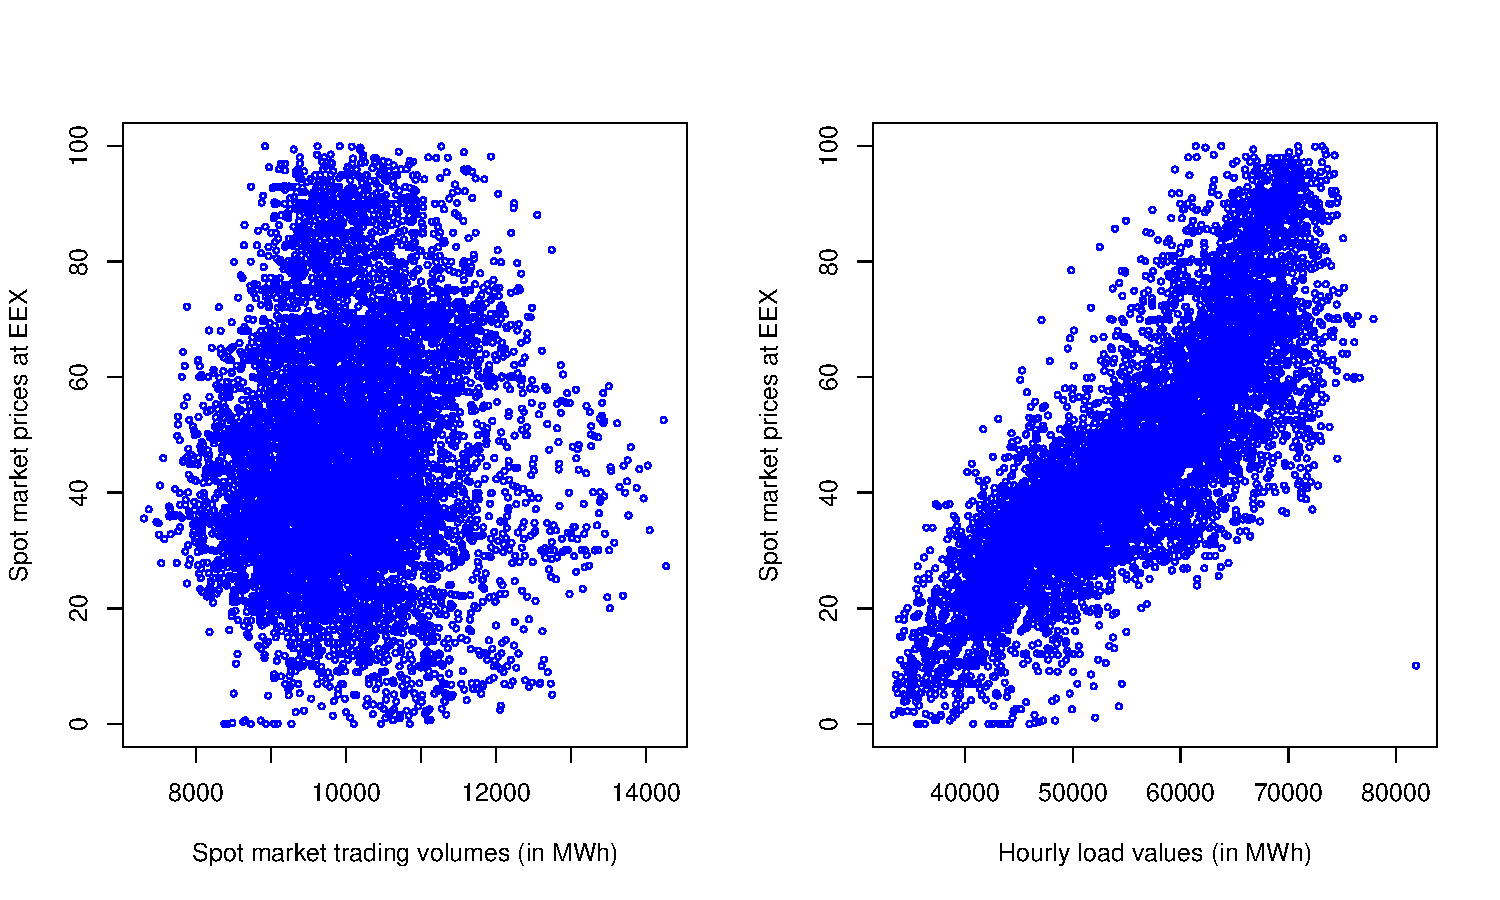
\includegraphics[width=3.5in]{germandata/pricequant.pdf}
  \label{fig:pricequant}
\\
 \scriptsize Source: EEX, UCTE
\end{figure}

To account for different states of the market, we separated the price-quantity combinations which occurred within a year by prices. As can be seen in Table \ref{tab:demand}, markets with extremely high prices occur only seldomly and prices between 20 and 40 are most common. For each of the six states in which the market might be we created linear demand functions based on average prices and quantities in these states. Note, that we also model the high-price market segment, to include price spikes which are a stylized fact of electricity prices.  To construct demand curves, \cite{Neuhoff2005} use a demand elasticity of 0.1, whereby \cite{Genc2007} argue that 0.2 is more commonly used to simulate the electricity market. As we have a more long run focus, we decided to use the latter value. It might be argued, that electricity demand is completely inelastic, as maybe only a very few industrial clients reduce their demand when prices rise. In response to that, \cite{Bushnell2003} notes that imports and exports provide some elasticity.

\begin{table}[htb]
\centering
\caption{Market segments}
\vspace{0.3cm}
\begin{tabular}{lrrr}
\hline
 & \multicolumn{1}{c}{Occupancy} & \multicolumn{1}{c}{Average price} & \multicolumn{1}{c}{Average quantity}   \\ 
 & \multicolumn{1}{c}{per year} & \multicolumn{1}{c}{(EUR)} & \multicolumn{1}{c}{(MWh)}   \\ 
 \hline
$>$ 100 & \multicolumn{1}{c}{46} & \multicolumn{1}{c}{128} & \multicolumn{1}{c}{83,558}   \\ 
between 80 and 100 & \multicolumn{1}{c}{134} & \multicolumn{1}{c}{86} & \multicolumn{1}{c}{81,493}   \\ 
between 60 and 80 & \multicolumn{1}{c}{788} & \multicolumn{1}{c}{68} & \multicolumn{1}{c}{78,256}   \\ 
between 40 and 60 & \multicolumn{1}{c}{2,174} & \multicolumn{1}{c}{49} & \multicolumn{1}{c}{71,956}  \\ 
between 20 and 40 & \multicolumn{1}{c}{4,201} & \multicolumn{1}{c}{30} & \multicolumn{1}{c}{58,578}  \\ 
below 20 & \multicolumn{1}{c}{1,417} & \multicolumn{1}{c}{14} & \multicolumn{1}{c}{42,627} \\
\hline
 & \multicolumn{1}{c}{8760} &  &    \\ 
 \hline
\end{tabular}
\label{tab:demand}
\\
\vspace{0.3cm}
\scriptsize Source: UCTE and EEX 
\end{table}

%\subsection{Supply}

Data concerning the short run marginal costs and investment costs per MWh were obtained from \cite{Auer2006} and are shown in Table \ref{tab:costs}. For pump storage plants we used the real option value of peak load electricity, which we approximated by the average option price for peak load electricity at the EEX in the year 2006. We do not provide fixed costs for pump hydropower and oil plants. In the case of hydropower plants construction costs depend heavily on the respective sites and therefore such costs are hard to estimate. Furthermore, all available sites for significant hydropower capacities in Central Europe seem to be occupied already. Oil fired plants are not considered a relevant investment option, because oil prices are just too high. The fixed investment costs can also be interpreted as present value of future yearly costs of capital.

\begin{table}[htb]
\centering
\caption{Variable and fixed costs}
\vspace{0.3cm}
\begin{tabular}{rrr}
\hline
           & Variable Costs & Investment Costs \\

           & (EURO/MWh) & EUROs per MWh \\
\hline
     Hydro &        7.6 &    3,500,000 \\

   Nuclear &        9.5 &    1,841,000 \\

   Lignite &       10.6 &    1,074,000 \\

 Hard Coal &       16.1 &     971,000 \\

CCGT &       33.5 &     460,000 \\

Oil & 44            &   n.a.\\
%Gas Turbines &       53.8 &     332000 \\

Pump Hydro &         80 &       n.a.\\
\hline
\end{tabular}
\label{tab:costs}
\\
\vspace{0.3cm}
\scriptsize Source: \cite{Auer2006}
\end{table}



%%% Local Variables: 
%%% mode: latex
%%% TeX-master: "../eem08"
%%% End: 
